\documentclass[]{article}
\usepackage[margin = 1.5in]{geometry}
\setlength{\parindent}{0in}
\usepackage{amsmath}
\usepackage{amsfonts}
\usepackage{amssymb}
\usepackage{amsthm}
\usepackage{pgfplots}

\usepackage{hyperref}
\usepackage[T1]{fontenc}
\usepackage{ae,aecompl}

\theoremstyle{definition}
\newtheorem{defn}{Definition}[section]
\newtheorem{ex}{Example}[section]

\setlength{\marginparwidth}{1.5in}
\newcommand{\lecture}[1]{\marginpar{{\footnotesize $\leftarrow$ \underline{#1}}}}

\begin{document}

	\title{\bf{CS 240: Data Structures and Data Management}}
	\date{Winter 2013, University of Waterloo \\ \center Notes written from Alejandro L\'opez-Ortiz's lectures.}
	\author{Chris Thomson}
	\maketitle
	\newpage

	\section{Introduction \& Code Optimization} \lecture{January 8, 2013}
		\subsection{Course Structure}
			The grading scheme is 50\% final, 25\% midterm, and 25\% assignments. There are five assignments, usually due on Wednesday mornings at 9:30 am. There are several textbooks for the course, all of which are optional but recommended. The textbooks cover roughly 80\% of the course content. There are also some course notes published online from previous terms, however the lectures will not necessarily follow those notes strictly.
			\\ \\
			See the \href{https://www.student.cs.uwaterloo.ca/~cs240/w13/info.phtml}{course syllabus} for more information.
			
		\subsection{CS as the Science of Information}
			So far in our undergraduate careers, computer science has meant programming. However, programming is only a subset of computer science. Computer science is the \textbf{science of information}.
			\\ \\
			What do we want to do with information? We want to:
			\begin{itemize}
				\item \textbf{Process it}. Programs $\equiv$ algorithms.
				\item \textbf{Store it}. We want to encode it. This also leads to information theory. Storing information involves data structures, databases, (file) systems, etc., all of which are searchable in some way.
				\item \textbf{Transmit it}. We want to transmit information over networks. This process involves coding theory.
				\item \textbf{Search it}. First, we have to structure it with data structures and/or SQL databases. Information retrieval is the process of searching for textual information instead of numerical information.
				\item \textbf{Mine it}. This involves artificial intelligence and machine learning.
				\item \textbf{Display it}. Information needs to be displayed using computer graphics (CG) and user interfaces (UI, partially related to psychology).
				\item \textbf{Secure it}. Encryption and cryptography are important. Information should also be stored redundantly to prevent harm from catastrophic events.
			\end{itemize}
	
		\subsection{Objectives of the Course}
			\begin{itemize}
				\begin{item}
					\textbf{Study efficient methods of storing, accessing, and performing operations on \underline{large} collections of data.} \\ \\
					``Large" is subjective -- your data needs to be large enough to justify the additional mental complexity. \\ \\
					Typical operations:
					\begin{itemize}
						\item Insert new item.
						\item ``Deleting" data (flagging data as ``deleted", not actually deleting the data).
						\item Searching for data.
						\item Sorting the data. \\
					\end{itemize}
				
					Examples of ``large data":
					\begin{itemize}
						\item The web.
						\item Facebook data.
						\item DNA data.
						\item LHC (Large Hadron Collider) measurements (terabytes per day).
						\item All the music from iTunes, for finding duplicate songs, etc.
					\end{itemize}
				\end{item}
				
				\begin{item}
					\textbf{There is a strong emphasis on mathematical analysis.} \\ \\
					The performance of algorithms will be analyzed using order notation.
				\end{item}
				
				\begin{item}
					\textbf{The course will involve abstract data types (objects) and data structures.} \\ \\
					We will see examples that have to do with:
					\begin{itemize}
						\item Databases.
						\item Geographic databases.
						\item Text searching.
						\item Text compression.
						\item Web searching.
					\end{itemize}
				\end{item}
			\end{itemize}
			
		\subsection{Code Optimization \& Measuring Performance}
			Richard Feynman was in charge of the computer group on the Manhattan Project. He made his code run 10x faster.
			\\ \\
			The initial method to measure performance was to use a \textbf{wall clock}. Initial studies looked like this:

			\begin{center}
				\begin{tabular}{|c|c|c|}
					\hline
					Data size & A & B \\ \hline
					3 & 1 & 3 \\
					5 & 2 & 9 \\
					10 & 4 & 10 \\
					20 & 16 & 11 \\ \hline
				\end{tabular}
			\end{center}
			
			However, computers were getting better, so we couldn't use wall clocks anymore. Results were not robust enough due to the qucik progression of performance increases in terms of computing power. Moreover, because of the differences in architecture, the same program may have a different execution time on two different computer models.
			\\ \\ 
			\underline{Idea}: rather than comparing algorithms using seconds, we should compare algorithms using the number of operations required for the algorithm to run.
			
			\begin{itemize}
				\item Express algorithm uisng pseudocode.
				\item Count the number of primitive operations.
				\item Plot the number of operations vs. the input size. \\
			\end{itemize}
			
			\begin{figure}
				\centering
				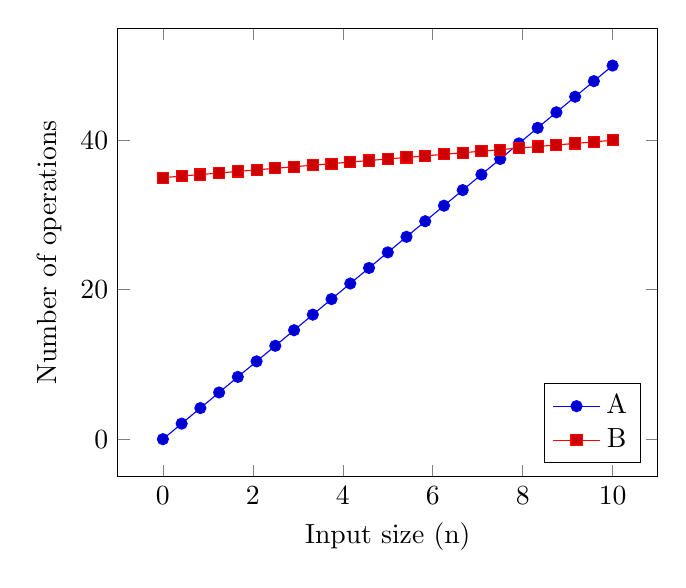
\begin{tikzpicture}[domain=0:10]
					\begin{axis}[
						xlabel = Input size (n),
						ylabel = Number of operations,
						legend entries = {A,B},
						legend pos = south east]
						\addplot{5*x};
						\addplot{0.5*x+35};
					\end{axis}
				\end{tikzpicture}
				\caption{A comparison of two algorithms $A$ and $B$.}
			\end{figure}
			
			Note that $A$ and $B$ are plotted as continuous functions, however they are not actually continuous -- we join all of the points for readability purposes only.
			\\ \\
			In the long run, you may want to use algorithm $B$ even if algorithm $A$ is better in some cases, because the benefits of $A$ will be short lived as $n$ grows.
			\\ \\
			Hence, comparing the programs has been transformed into comparing functions. We use order notation to measure the long-term growth of functions, allowing us to choose the smaller function, which corresponds to the faster algorithm.
	
	\section{Order Notation} \lecture{January 10, 2013}
		The time for algorithm $A$ on input of size $n$ is:
		
		\begin{align*}
			\underbrace{2n \log n}_\text{sort} + \underbrace{1.5n^3}_\text{mult} + \underbrace{22n^2 - 3n}_\text{additions} + \underbrace{7}_\text{setup}
		\end{align*}
		
		On a different machine, the same algorithm $A$ may be $2n \log n + 9n^3 + 10n^2 - 3n + 7$. These give a \textbf{false sense of precision}. These specifics can also be quite costly to determine. In the 1960s, Don Knuth proposed \textbf{order notation} as a way to analyze the general quality of algorithms in an accurate, cost- and time-efficient way by ignoring precise runtimes.
		
		\subsection{Formal Definitions}
			Order notation represents algorithms as functions. We say a function $f(n)$ relates to a certain order $g(n)$ using different notation depending on which relation we're interested in.
			\begin{center}
				\begin{tabular}{|c|c|}
					\hline
					 Relation & Functions \\ \hline
					 $3 \le 7$ & $f(n) = O(g(n))$ \\
					 $8 \ge 7$ & $f(n) = \Omega(g(n))$ \\
					 $7 = 7$ & $f(n) = \Theta(g(n))$ \\
					 $3 < 7$ & $f(n) = o(g(n))$ \\
					 $7 > 3$ & $f(n) = \omega(g(n))$ \\ \hline
				\end{tabular}
			\end{center}
			
			Here's an easy way to remember the correspondence between a relation and its order notation symbol: the greedy operators, $\le$ and $\ge$, are uppercase letters $O$ and $\Omega$. The less greedy operators, $<$ and $>$, are the same letters but in lowercase ($o$ and $\omega$). \\
			
			Order notation only cares about the long run. An algorithm can violate the relation early -- we're interested in its asymptotic behaviour.
			
			\begin{defn}[$\le$]
				$f(n) = O(g(n))$ if there exist constants $c > 0, n_0 > 0$ such that $f(n) \le c \cdot g(n)$ for all $n \ge n_0$.
			\end{defn}
		
			\begin{defn}[$\ge$]
				$f(n) = \Omega(g(n))$ if there exist constants $c > 0, n_0 > 0$ such that $f(n) \ge c \cdot g(n)$ for all $n \ge n_0$.
			\end{defn}
			
			\begin{defn}[$=$]
				$f(n) = \Theta(g(n))$ if there exists constants $c_1, c_2 > 0$ such that $c_1 \cdot g(n) \le f(n) \le c_2 \cdot g(n)$.
			\end{defn}
			
			The equality relation is effectively sandwiching the algorithm $f(n)$ between two other functions (the squeeze theorem). If it's possible to sandwich the algorithm between two multiples of the same $g(n)$, then $f(x)$ is said to be equal to the order $g(n)$.
			
			\begin{defn}[$<$]
				$f(n) = o(g(n))$ if for all $c > 0$ there exists constant $n_0 > 0$ such that $f(n) < c \cdot g(n)$ for all $n \ge n_0$.
			\end{defn}
		
			\begin{defn}[$>$]
				$f(n) = \omega(g(n))$ if for all $c > 0$ there exists constant $n_0 > 0$ such that $f(n) > c \cdot g(n)$ for all $n \ge n_0$.
			\end{defn}
			
		\subsection{Order Notation Examples}
			\begin{ex}
				$2n^2 + 3n + 11 = O(n^2)$
				\\ \\
				We need to show that there exists constants $c > 0$ and $n_0 > 0$ such that $2n^2 + 3n + 11 \le cn^2$ for all $n \ge n_0$.
				\\ \\
				Let $c = 3$. Simplifying gets us $3n + 11 \le n^2$. This holds for $n_0 = 1000$, for instance.
			\end{ex}
			
			\begin{ex}
				$2n^2 + 3n + 11 1 = \Theta(n^2)$
				\\ \\
				In order to show equality ($\Theta$), we need to show both the $\le$ and $\ge$ cases. In the previous example, the $\le$ case was shown. For the $\ge$ case, we need to show $n^2 \le c \cdot (2n^2 + 3n + 11)$.
				\\ \\
				Let $c = 1$. Simplifying gets us $n^2 \le 2n^2 + 3n + 11$, which gives us $0 \le n^2 + 3n + 11$. This holds for $n_0 = 0$.
			\end{ex}
			
			\begin{ex}
				$2010n^2 + 1388 = o(n^3)$
				\\ \\
				We must show that for all $c > 0$, there exists $n_0 > 0$ such that $2010n^2 + 1388 \le c \cdot n^3$ for all $n \ge n_0$.
				
				\begin{align*}
					\frac{2010n^2+1388}{n^3} \stackrel{?}{\le} \frac{c \cdot n^3}{n^3} \implies \frac{2010}{n} + \frac{1388}{n^3} \stackrel{?}{\le} c
				\end{align*}
				
				There is a \textbf{trick to prove f(n) = o(g(n))}: show that $\lim_{n \to \infty}{}\frac{f(n)}{g(n)} = 0$.
			\end{ex}
		
		\subsection{A note about the use of =}
			\begin{align*}
				\underbrace{2n^2}_\text{specific function} \in \underbrace{O(n^2))}_\text{set of functions}
			\end{align*}
			
			The use of the equality operator ($=$) in order notation is not the same as in most other areas of mathematics, since a single element of a set cannot strictly be equal to the set itself (even $a \ne \{a\}$). The $=$ in order notation is not a true equality -- it's just notation. The $\in$ operator is semantically more correct.
		
		\subsection{Performance of Algorithms}
			We have made some progression in how we determine the performance of algorithms.
			\begin{itemize}
				\item Comparing single runs.
				\item Comparing measured curves (multiple runs).
				\item Produce analytical expressions for the curves.
				\item Simplify using order notation.
			\end{itemize}
			
			Let's say we have the problem of integrating a mathematical function. Our program numerically integrates the function, and we're trying to analyze the algorithm behind that process. The timing would vary depending on the mathematical function and precise required.
			\\ \\
			If we conduct multiple runs of our algorithm, we'll get different times. Plotting all of the results (time vs. input size) will result in data that is not a function, because the data fails the vertical line test, since for a given input size we have multiple times.
			\\ \\
			We need to decide on a convention for these cases where we have multiple time values. In this course, we'll usually look at the worst case, however in some situations examining the best or average cases could be useful.
			\\ \\
			Finding the average case is hard. To produce an appropriate average, we need an input distribution.
\end{document}